\documentclass[t]{beamer}

\mode<presentation>
{
  \usetheme{default}
  \setbeamertemplate{navigation symbols}{}
  \setbeamertemplate{footline}[frame number]
  \setbeamertemplate{items}[circle]
  \usecolortheme{seahorse}
}

\usepackage[english]{babel}
\usepackage[utf8]{inputenc}
\usepackage{times}
\usepackage[T1]{fontenc}
\usepackage{url}
\usepackage[]{algorithm2e}
\usepackage{amsmath}
\usepackage{centernot}
\usepackage{xcolor}

\parskip=8 pt

\newcommand\topstrut{\rule{0pt}{2.6ex}}
\newcommand\bottomstrut{\rule[-1.2ex]{0pt}{0pt}}
\newcommand\doublestrut{\rule[-1.2ex]{0pt}{3.6ex}}

\newcommand\blue[1]{\textcolor{blue}{#1}}
\newcommand\red[1]{\textcolor{red}{#1}}
\newcommand\gray[1]{\textcolor{gray}{#1}}
\newcommand\smallgray[1]{\textcolor{gray}{\small\it #1}}
\newcommand\prevwork[1]{\smallgray{#1}}

\title
{Cette présentation pourrait vous intéresser\dots}
\subtitle{Une introduction aux moteurs de recommendation}

\author[Abrahamson] {Jeff Abrahamson}\institute{Jellybooks}

\date[7 novembre 2014]
%{Nantes Machine Learning Meetup, 3 novembre 2014}

% Delete this, if you do not want the table of contents to pop up at
% the beginning of each subsection:
\AtBeginSubsection[]
{
  \begin{frame}<beamer>{Outline}
    \tableofcontents[currentsection,currentsubsection]
  \end{frame}
}

% If you wish to uncover everything in a step-wise fashion, uncomment
% the following command: 
%\beamerdefaultoverlayspecification{<+->}

\begin{document}

\begin{frame}
  
\includegraphics[width=\textwidth]{2014_affiche_A2_paysage_avec_sponsors.png}
  
  \centerline{\fcolorbox{purple}{pink}{\blue{ici : moteurs de recommandation}}}
\end{frame}

\begin{frame}
  \titlepage
\end{frame}

\begin{frame}
  \frametitle{Définition}

  \vspace{2cm}
  
  \centerline{\parbox{.8\textwidth}{ Étant donné information sur
      l'utilisateur, son environnement, et des objets d'intérêt,
      déterminer les objets recommandables les plus pertinents.}}

  \vspace{1cm}
  \only<2>{
    On n'est pas contraint à trouver les $\max k$.

    Il suffit de trouver $k$ parmi un $\max n$.
  }
\end{frame}

%% TODO -- lots of images

\begin{frame}
  \frametitle{Exemples}
  \begin{itemize}
  \item Amazon
  \item Google News (ou Le Monde)
  \item Facebook
  \item Diagnostique médicale
  \item App Store / Google Play
  \item Youtube
  \item Publicités
  \item Netflix, last.fm, Spotify, Pandora, \dots
  \item Browser (propositions de URL)
  \item Recherche
  \end{itemize}
  % TODO: images
\end{frame}

\begin{frame}
  \frametitle{Valeur pour le client}
  \begin{itemize}
  \item Trouver --- intéressant
  \item Réduire choix
  \item Explorer options
  \item Découverte (``long tail'')
  \item Loisirs
  \end{itemize}
\end{frame}

\begin{frame}
  \frametitle{Valeur pour le fournisseur}

  \begin{itemize}
  \item Prestation unique / supplémentaire
  \item Confiance, fidélité
  \item Augmenter ventes, CTR, conversions
  \item Mieux comprendre le client
  \end{itemize}
\end{frame}

%% TODO - slide, image of jumping around
\begin{frame}
  \frametitle{Attacher vos ceintures\dots}

  \begin{itemize}
  \item On va beaucoup sauter
  \item Il restera des trous
  \item Trop de matériel, rien n'est vrai tout le temp
  \item<2> \gray{Tout projet est un projet de recherche}
  \item<3> Tout projet est un projet de recherche
  \item<3> \blue{Objectif : plus de perspectif}
  \end{itemize}
\end{frame}

% ======================================================================
% Technique Overview

\begin{frame}
  \frametitle{La recommendation}

  \begin{tabular}{|p{5.7cm}|p{4cm}|}
    \hline
    \topstrut\hbox{Content-based filtering}
    \hbox{\it (filtrage basée sur le continu)}
    &
    Plus de ce qui ressemble à ce que j'aime.\bottomstrut
    \\
    \hline
    \topstrut\hbox{Collaborative filtering}
    \hbox{\it (filtrage collaboratif)}
    &
    Plus de ce que d'autres qui aiment ce que j'aime aiment.\bottomstrut
    \\
    \hline
    \topstrut\hbox{Knowledge-based filtering}
    \hbox{\it (filtrage basée sur connaissance)}\bottomstrut
    &
    Plus de ce qu'il faut.\bottomstrut
    \\
    \hline
  \end{tabular}
\end{frame}

\begin{frame}
  \frametitle{Content-based filtering}

  Pour
  \begin{itemize}
  \item Pas besoin de communauté
  \item Comparaison entre objets possible.
  \end{itemize}

  \bigskip
  Contre :
  \begin{itemize}
  \item Comprendre contenu
  \item Cold start (nouveaux utilisateurs)
  \item Pas de sérendipité
  \end{itemize}
\end{frame}

\begin{frame}
  \frametitle{Collaborative filtering}

  Pour
  \begin{itemize}
  \item Sans études du contenu
  \item Sérendipité
  \item Apprentissage du marché
  \end{itemize}

  \bigskip
  Contre :
  \begin{itemize}
  \item Retours des utilisateurs
  \item Cold start (nouveaux utilisateurs)
  \item Cold start (nouveaux objects)
  \end{itemize}
\end{frame}

\begin{frame}
  \frametitle{Knowledge-based filtering}

  Pour
  \begin{itemize}
  \item Déterministe
  \item Sûr
  \item Pas de cold start
  \item Expertise commerciale
  \end{itemize}

  \bigskip
  Contre :
  \begin{itemize}
  \item Étude pour bootstrap
  \item Statique, ne répond pas aux tendances
  \end{itemize}

  \only<2>{\bigskip \blue{On n'en parle plus.}}
\end{frame}


% ======================================================================
% Linear Algebra Basics

\begin{frame}
  \frametitle{Utility Matrix}

  \begin{itemize}
  \item Users (utilisateurs)
  \item Items (objets)
  \end{itemize}

  \only<2->{Le but est de trouver les blancs.}

  \only<2>{
    \vspace{1cm}
    \centerline{\begin{tabular}{l|ccccc}
        & $I_1$ & $I_2$ & $I_3$ & $I_4$ & $I_5$ \\
        \hline
        $U_1$ & 1 & & & & \\
        $U_2$ & & & 1 & 1 & 1 \\
        $U_3$ & & 1 & & 1 & 1
      \end{tabular}}

    \bigskip
    \centerline{\gray{Par exemple, vente de livres chez Amazon.}}
  }
  \only<3>{
    \vspace{1cm}
    \centerline{\begin{tabular}{l|ccccc}
        & $I_1$ & $I_2$ & $I_3$ & $I_4$ & $I_5$ \\
        \hline
        $U_1$ & 3 & & & & \\
        $U_2$ & & & 5 & 1 & 4 \\
        $U_3$ & & 2 & & 5 & 1
      \end{tabular}}

    \bigskip
    \centerline{\gray{Par exemple, avis de filmes à Netflix.}}
  }

  \only<2->{
    \bigskip
    \gray{\it Mais des milliers ou des millions de colonnes et de lignes.}
  }
\end{frame}

\begin{frame}
  \frametitle{Utility Matrix}

  D'où viennent la matrice ?
  \begin{itemize}
  \item Demande aux utilisateurs
  \item Observer nos utilisateurs
  \end{itemize}

  Ça peut coûter cher\dots
\end{frame}

\begin{frame}
  \frametitle{Item Profiles}

  Exemples :
  \begin{itemize}
  \item Filmes \gray{$\qquad\Rightarrow$ ?}
  \item Livres \gray{$\qquad\Rightarrow$ ?}
  \item Actualités \gray{$\qquad\Rightarrow$ ?}
  \item Images \gray{$\qquad\Rightarrow$ ?}
  \end{itemize}

  \only<2>{\gray{ Filmes :}

    \gray{Contenu : acteurs, cinéaste, année (décennie, etc.), durée}

    \gray{Collaboratif : vu, avis~(1--5), ou vu, quand vu relatif à sa sortie}
  }
  \only<3>{\gray{Livres :}

    \gray{Contenu : auteur, genre, année (décennie, etc.), nombre de
      pages, contenu (très difficile)}

    \gray{Collaboratif : lu, avis~(1--5), comment lu}
  }
  \only<4>{\gray{Actualités :}

    \gray{Contenu : source, section, vecteurs de mots avec TF-IDF
      important}

    \gray{Collaboratif : }
  }
  \only<5>{\gray{Images :}

    \gray{Contenu :}

    \gray{Collaboratif :}
  }
  
  \only<6>{

    \gray{Et puis profils d'utilisateur.}

    \gray{Le comportement de l'utilisateur lui attribue des composants
      des vecteurs.}
  }

\end{frame}

\begin{frame}
  \frametitle{Similarité : Indice de Jaccard}

  ou : \textit{Jaccard index}, \textit{Jaccard similarity coefficient}
  
  \vspace{1cm}
  Similarité :
  \begin{displaymath}
    J(A,B) = \frac{|A\cap B|}{|A\cup B|}
  \end{displaymath}

  \only<2>{
    Distance :
    \begin{displaymath}
      J_{\delta}(A,B) = 1 - J(A,B)
    \end{displaymath}
  }
\end{frame}

\begin{frame}
  \frametitle{Similarité cosinus}

  ou : mesure cosinus, \textit{cosine similarity}

  \vspace{1cm}
  Similarité :
  \only<1>{
    \begin{displaymath}
      \cos \theta = \frac{A\cdot B}{\parallel A\parallel \parallel B\parallel}
    \end{displaymath}
  }
  \only<2->{
    \begin{displaymath}
      S_C(A,B) = \frac{A\cdot B}{\parallel A\parallel \parallel B\parallel}
    \end{displaymath}
  }
  
  \only<3->{
    Distance :
    \begin{displaymath}
      D_C(A,B) = 1-S_C(A,B)
    \end{displaymath}
  }

  \only<4>{
    \blue{On ne prend que les composants non-vides.}
  }
\end{frame}

\begin{frame}
  \frametitle{Textes : TF-IDF}
  
  \begin{itemize}
  \item Vecteurs de fréquences de mots
  \item Fréquence $\centernot\implies$ significance
  \item<2> Term Frequency - Inverse Document Frequency
  \end{itemize}
\end{frame}

\begin{frame}
  \frametitle{Textes : TF-IDF}

  \begin{displaymath}
        TF_{ij} = \frac{f_{ij}}{\max_k f_{kj}} \qquad\qquad
        IDF_I = \log_2\left( \frac{N}{n_i} \right)
  \end{displaymath}
  
  \begin{displaymath}
        TF\mbox{-}IDF_{ij} = TF_{ij} \cdot IDF_i
  \end{displaymath}

  avec :
  \begin{align*}
    f_{ij} &= \mbox{fréquence de mot $i$ dans document $j$} \\
    N &= \mbox{nombre de document}\\
    n_i &= \mbox{nombre de document dans lesquels on trouve terme $i$}
  \end{align*}

  
  \only<2->{
    IDF est une mesure de l'information que porte un mot.

    TF-IDF nous dit quels mots caractérisent le mieux le document.
  }
  
  \only<3>{
    \vspace{-5mm}
    \gray{Variation : boolean, log, filtrage de mots vide}
  }
\end{frame}


% ======================================================================
% Item-Item Filters

\begin{frame}
  \frametitle{Content-Based Filtering}

  \vspace{1cm}

  \vspace{15mm} % A fragile hack.
  \centerline{\fcolorbox{blue}{white}{\hspace{55mm}\rule{0pt}{1.45ex}}}
  \vspace{-15mm}
  
  \centerline{\begin{tabular}{l|ccccc}
      & $I_1$ & $I_2$ & $I_3$ & $I_4$ & $I_5$ \\
      \hline
      $U_1$ & 3 & & & & \\
      $U_2$ & & & 5 & 1 & 4 \\
      $U_3$ & & 2 & & 5 & 1
    \end{tabular}}

  \vspace{1cm}
  \centerline{Plus de ce qui ressemble à ce que j'aime}

  \only<2>{
    \vspace{1cm}
    \gray{Et puis, partitionnement de données (regroupement, \textit{clustering}),
      etc.}
  }
\end{frame}

\begin{frame}
  \frametitle{Content-Based Filtering}

  % TODO: Define this
  % TODO: Item-Item Filters
  
  Basé sur les profils d'objets (\textit{item profiles})
  \begin{itemize}
  \item Plus stable (en principe)
  \item $O(n^2)$ (mais souvent moins, objets sans co-classement)
  \item Peut réduire le seuil
  \item Pré-calcul possible, requête (plus) rapide
  \end{itemize}
\end{frame}


% ======================================================================
% Collaborative Filters

\begin{frame}
  \frametitle{Collaborative Filtering}

  \vspace{1cm}
  \centerline{\begin{tabular}{l|ccccc}
      & $I_1$ & $I_2$ & $I_3$ & $I_4$ & $I_5$ \\
      \hline
      $U_1$ & 3 & & \fcolorbox{blue}{white}{4} & \fcolorbox{blue}{white}{2} & \\
      \fcolorbox{blue}{white}{$U_2$} & & & 5 & 1 & 4 \\
      $U_3$ & & 2 & & 5 & 1
    \end{tabular}}

  \vspace{1cm}
  \centerline{Plus de ce que d'autres qui aiment ce que j'aime aiment.}
\end{frame}

\begin{frame}
  \frametitle{Collaborative Filtering}

  \vspace{1cm}
  
  \vspace{15mm} % A fragile hack.
  \centerline{\fcolorbox{blue}{white}{\hspace{55mm}\rule{0pt}{1.45ex}}}
  \vspace{-15mm}
  
  \centerline{\begin{tabular}{l|ccccc}
      & $I_1$ & $I_2$ & $I_3$ & $I_4$ & $I_5$ \\
      \hline
      $U_1$ & 3 & & & & \\
      $U_2$ & & & 5 & 1 & 4 \\
      $U_3$ & & 2 & & 5 & 1
    \end{tabular}}

  \vspace{1cm}
  Le Profil d'utilisateur.
\end{frame}

\begin{frame}
  \frametitle{Collaborative Filtering}

  \vspace{1cm}
  
  % A fragile hack.
  \vspace{19mm}
  \centerline{\hspace{8mm}\fcolorbox{blue}{white}{\hbox to 10pt{\vbox to 19mm{}}}}
  \vspace{-20mm}
  
  \centerline{\begin{tabular}{l|ccccc}
      & $I_1$ & $I_2$ & $I_3$ & $I_4$ & $I_5$ \\
      \hline
      $U_1$ & 3 & & 4 & 2 & \\
      $U_2$ & & & 5 & 1 & 4 \\
      $U_3$ & & 2 & & 5 & 1
    \end{tabular}}

  \vspace{1cm}
  Le Profil d'objet.
\end{frame}

\begin{frame}
  \frametitle{Utility Matrix Symmetry}

  \begin{itemize}
  \item Proposer d'objets basés sur des utilisateurs
  \item Proposer d'utilisateurs basés sur des objets
  \end{itemize}

  \only<2>{Mais, par exemple : 2 objets similaire $\,\centernot\equiv\,$ 2 utilisateurs
      similaires.}
  \only<3>{
      Pour estimer $m_{u,i}$,
      \begin{itemize}
      \item Trouver $k$ utilisateur comme $U_u$
      \item Trouver $k$ objets comme $I_i$
      \end{itemize}
    }
\end{frame}

\begin{frame}
  \frametitle{Utility Matrix : Estimer $m_{u,i}$}

  \vspace{1cm}
  \centerline{\begin{tabular}{l|ccccc}
      & $I_1$ & $I_2$ & $I_3$ & $I_4$ & $I_5$ \\
      \hline
      $U_1$ & 3 & & 4 & 2 & \fcolorbox{blue}{white}{\rule{0pt}{.9ex}\ }\\
      $U_2$ & & & 5 & 1 & 4 \\
      $U_3$ & & 2 & & 2 & 3
    \end{tabular}}

  \bigskip
  \begin{itemize}
  \item Trouver $k$ utilisateur comme $U_u$, prendre $\frac{1}{k}
    \sum_{j=1}^k m_{u_j,i}$
  \item Trouver $k$ objets comme $I_i$, prendre $\frac{1}{k}
    \sum_{j=1}^k m_{u,i_j}$
  \end{itemize}

  \only<2>{
    \gray{Il faut calculer la ligne complète (ou la partie qui est
      susceptible d'être important)}
  }
  \only<3>{
    \gray{Une fois pour $U_u$, les $k$ autres nous donne un
      raccourcis.}

    \gray{Pour $I_i$, il faut calculer presque tous les $I_j$ avant de
      pouvoir remplir une seule ligne.  Par contre, objet-objet
      souvent plus fiable (exemple de genre d'objet / genre de personne).}
  }
  \only<4>{
    \gray{En tout cas, on fait la plupart en avance.}
  }
\end{frame}

\begin{frame}
  \frametitle{Utility Matrix}

  La matrice est creuse.

  $\implies$ clustering $\implies$ matrice réduites

  \only<2>{\gray{Estimation sur la matrice réduite, puis prendre
      d'objets et d'utilisateurs représentatif dans le
      \textit{cluster} (paquet).
    }}

\end{frame}


% ======================================================================
% Amazon's Item-Item Filter

\begin{frame}
  \frametitle{Amazon : Item-to-Item Collaborative Filtering}

  Observations :
  \vspace{1cm}

  \centerline{
    \only<1>{\textit{Clustering} coûte cher, diminue qualité}
    \only<2>{\textit{Dimension reduction} diminue qualité}
    \only<3>{Utilisateurs touchent peu d'objets}
    \only<4>{Réponse rapide désirable}
  }
\end{frame}

\begin{frame}
  \frametitle{Amazon : Item-to-Item Collaborative Filtering}

  Scale indépendemment du nombre d'utilisateur et du nombre d'objets
  \begin{itemize}
  \item Online
  \item Offline
  \end{itemize}

  \bigskip
  \gray{G.~Linden, B.~Smith, J.~York, \textit{Amazon.com
      Recommendations: Item-to-Item Collaborative Filtering}, Internet
  Computing (7, 1), 22 Jan 2003.}

\end{frame}

\begin{frame}
  \frametitle{Amazon : Item-to-Item Collaborative Filtering}
  Offline (Precomputation)

  \DontPrintSemicolon
  \begin{algorithm}[H]
    \For{chaque objet $I_1$ à vendre}{
      \For{chaque utilisateur $C$ qui a acheté $I_1$}{
        \For{chaque objet $I_2$ acheté par $C$}{
          $(I_1,I_2)$++\;
        }
      }
      \For{chaque object $I_2$}{
        $S_{I_1,I_2} \gets S(I_1,I_2)$\;
      }
    }
  \end{algorithm}
\end{frame}


% ======================================================================
% Slope One

\begin{frame}
  \frametitle{Slope One}

  \vspace{1cm}
  Régression linéaire sur les avis des utilisateurs.
  \vspace{1cm}
  
  \gray{Daniel Lemire and Anna Maclachlan, \textit{Slope One
      Predictors for Online Rating-Based Collaborative
      Filtering},Proceedings of SIAM Data Mining (SDM) 2005.}
\end{frame}

\begin{frame}
  \frametitle{Slope One : Régression}

  \vspace{1cm}
  \centerline{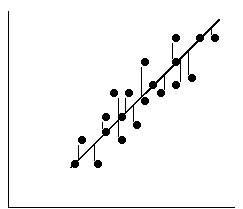
\includegraphics[height=.4\textheight]{regression.png}}

  \only<2>{
    \begin{displaymath}
      \min \sum (y_i-(ax_i+b))^2
    \end{displaymath}
    \vspace{1mm}
  }
  \vspace{1cm}
  \centerline{\gray{\footnotesize \url{http://www.upa.pdx.edu/IOA/newsom/pa551/Image255.gif}}}
  
\end{frame}

\begin{frame}
  \frametitle{Slope One : algorithme}

  Offline :
  \DontPrintSemicolon
  \begin{algorithm}[H]
    \For{chaque $I_i$, $I_j$}{
      $\mathcal{U} \gets \{\mbox{utilisateurs qui ont exprimé un avis
        sur } I_i, I_j \} $\;
      $\mbox{dev}_{i,j} \gets \frac{1}{\parallel\mathcal{U}\parallel}
      \sum_{u\in\mathcal{U}} (r_u(i) - r_u(j))$ \;
    }
  \end{algorithm}
  \bigskip
    Online (pour $u$) :
  \DontPrintSemicolon
  \begin{algorithm}[H]
    $\mathcal{V} \gets \{ j \mid u \mbox{ a exprimé un avis
      sur } I_j \} $\;
    $r_u(i) \gets \frac{1}{\parallel\mathcal{V}\parallel}
    \sum_{u\in\mathcal{V}} (\mbox{dev}_{i,j} - r_u(j))$ \;
  \end{algorithm}


\end{frame}

\begin{frame}
  \frametitle{Slope One : Régression}
  
  \vspace{1cm}
  \centerline{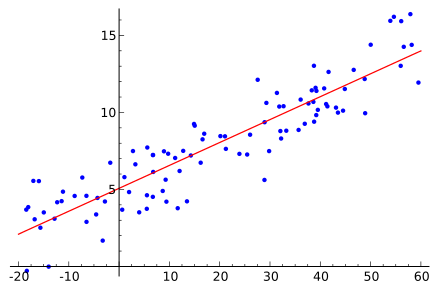
\includegraphics[height=.4\textheight]{linear-regression.png}}

  \vspace{1cm}
  \gray{\small "Linear regression" by Sewaqu - Own work. Licensed
    under Public domain via Wikimedia Commons -
    {\footnotesize\url{http://commons.wikimedia.org/wiki/File:Linear\_regression.svg\#mediaviewer/File:Linear_regression.svg}}}

\end{frame}

\begin{frame}
  \frametitle{Slope One : Régression}
  
  \vspace{1cm}
  \centerline{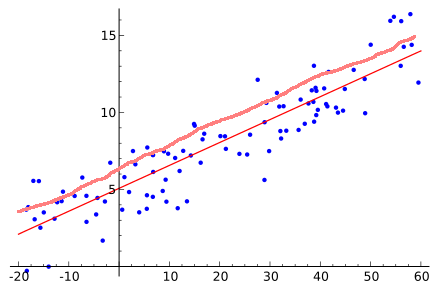
\includegraphics[height=.4\textheight]{linear-regression-2.png}}

\end{frame}


% ======================================================================
% Dimensionality Reduction

\begin{frame}
  \frametitle{Dimensionality reduction}

  SVD, $k=20\ldots 100$ typiquement

  Décomposition en valeurs singulières

  \only<1>{
    \begin{displaymath}
      M = U\Sigma V^*
    \end{displaymath}
  }
  \only<2>{
    \begin{displaymath}
      \begin{pmatrix}
        a_1 & \cdots & a_m
      \end{pmatrix}
      \begin{pmatrix}
        b_1 \\ \vdots \\ b_n
      \end{pmatrix} = \mathrm{scalaire} 
    \end{displaymath}
  }
  \only<3>{
    \begin{displaymath}
      \begin{pmatrix}
        a_1 \\ \vdots \\ a_m
      \end{pmatrix}
      \begin{pmatrix}
        b_1 & \cdots & b_n
      \end{pmatrix} =
      \begin{pmatrix}
        c_{1,1} & \cdots & c_{1,n} \\
        \vdots & & \vdots \\
        c_{m,1} & \cdots & c_{m,n}
      \end{pmatrix}
    \end{displaymath}
  }
  \only<4>{
    \begin{displaymath}
      \begin{pmatrix}
        a_{1,1} & a_{1,2} & a_{1,3} \\
        \vdots & \vdots & \vdots \\
        a_{m,1} & a_{m,2} & a_{m,3}
      \end{pmatrix}
      \begin{pmatrix}
        b_{1,1} & \cdots & b_{1,n} \\
        b_{2,1} & \cdots & b_{2,n} \\
        b_{3,1} & \cdots & b_{3,n}
      \end{pmatrix} =
      \begin{pmatrix}
        c_{1,1} & \cdots & c_{1,n} \\
        \vdots & & \vdots \\
        c_{m,1} & \cdots & c_{m,n}
      \end{pmatrix}
    \end{displaymath}
  }
  \only<5>{
    \begin{displaymath}
      \begin{pmatrix}
        a_{1,1} & \cdots & a_{1,k} \\
        \vdots & & \vdots \\
        a_{m,1} & \cdots & a_{m,k}
      \end{pmatrix}
      \begin{pmatrix}
        c_{1,1} & \cdots & c_{1,n} \\
        \vdots & & \vdots \\
        c_{k,1} & \cdots & c_{k,n}
      \end{pmatrix} =
      \begin{pmatrix}
        c_{1,1} & \cdots & c_{1,n} \\
        \vdots & & \vdots \\
        c_{m,1} & \cdots & c_{m,n}
      \end{pmatrix}
    \end{displaymath}
  }
  
\end{frame}

\begin{frame}
  \frametitle{Problèmes particuliers}

  \begin{itemize}
  \item Comment mesurer la réussite ?
  \item Quelles sont des critères ?
  \end{itemize}
\end{frame}

\begin{frame}
  \frametitle{Clustering}

  \begin{itemize}
  \item kNN \only<2>{\gray{$k$-Nearest Neighbor}}
  \item Curse of Dimensionality \only<2>{\gray{Fléau (ou :
        malédiction) de la dimension}}
  \item Scalabilité \only<2>{\gray{$10^7$ clients, $10^6$ objets}}
  \end{itemize}
\end{frame}


% ======================================================================
% End

\begin{frame}
  \frametitle{Questions ?}

  \vspace{1cm}
  \centerline{Sondage : \url{purple.com/devfest}}

  \vspace{1cm}
  \centerline{Et si vous êtes de la région, rdv sur meetup.com :}

  \bigskip
  \centerline{Nantes Machine Learning Meetup}
\end{frame}


\end{document}
